% !TEX root = ./cvl.tex
\section{Experimental Results}
\label{sec:experimental}

\marcos{What are the goals of the experiments? Certainly related to performance breakdown, quality, scalability, showing feasibility of very large datasets. The goals should motivate and reflect Sections~\ref{sec:exp:points} to~\ref{sec:exp:large} below.}
\marcos{Show three/four main sections and plots, explain all of them, justify effects observed.}
\martin{Compare experimental results with theory e.g. expected approximation guarantee, number of constraints, number of records per constraint etc.}

\subsection{Experimental Setup}

\minisec{Datasets}
We have tested CVL using four real-world datasets with the biggest one containing 23 million points and one synthetic dataset containing 30 million points. The airports dataset is from Openflights and contains 7411 airports (points). The tourism dataset contains 500 thousand points representing tourist attractions worldwide from the OpenStreetMap database. The fractal dataset (synthetic) was created by iteratively copying and displacing points from the tourism dataset within a 10km radius until 30 million records were reached. The US rivers/streams dataset contains 30 thousand named rivers and streams in the United States as multilinestrings, and has been reduced from a OpenStreetMap waterway dataset by merging objects with the same name into one. In the original dataset, most rivers are represented by multiple records, which is unfortunate in a filtering situation. The Protection zones dataset contains 30 thousand high-fidelity administrative protection zone polygons published by the Danish government, and ranges from small polygons the size of buildings to large polygons the size of entire regions.

\begin{table}[htdp]
\caption{Datasets used in experiments}
\begin{center}
\begin{tabular}{|c|c|c|c|c|}
\hline
\textbf{Origin} & \textbf{Dataset} & \textbf{Type} & \textbf{Records} & \textbf{Points} \\
\hline
Real & Airports & Points & $7K$ & $7K$ \\
Real & Tourism & Points & $500K$ & $500K$ \\
Synthetic & Fractal & Points & $30M$ & $30M$ \\
Real & US rivers/streams & Linestrings & $4K$ & $23M$ \\
Real & Proctection zones & Polygons & $30K$ & $9M$ \\
\hline
\end{tabular}
\end{center}
\label{default}
\end{table}%


\minisec{Hardware, Software, and Methods}
The hardware used for testing was an Amazon EC2 instance with 17GB RAM, 2 x Intel(R) Xeon(R) CPU E5-2665 0 @ 2.40GHz and 20MB Cache. 

The operating system was Amazon Linux 3.4.48-45.46.amzn1.x86\_64. An image of the instance we used for testing is available through Amazon EC2 as an AMI. The image contains the exact database used for testing, with all tables preloaded.

The database used for testing was PostgreSQL 9.2.4 with PostGIS  2.0. We used the following versions of libraries: GDAL 1.9.2 and GEOS 3.3.8. For the LP solver we integrated the database with the convex optimization library CVXOPT version 1.1.6 (\texttt{http://cvxopt.org/}). We installed Python language bindings in the database installed against Python 2.6.8.

We ran each test three times on this installation, taking the average of these runs. We observed that measurements were very stable, with negligible difference in compute time between runs.

It should be noted that PostgreSQL always uses a single core to compute a transaction. The generalization process in CVL is run as a single long transaction, which then means that the process is essentially run on a single core. A future avenue would be to investigate parallel executing as the structure of the single-scale filtering problem offers many opportunities for data parallelism.

\subsection{Point Data}
\label{sec:exp:points}

In this section, we present experimental results with point datasets, namely the Openflight airports and Tourist attractions datasets. We first discuss performance and quality breakdowns for CVL and then proceed to analyze CVL's scalability behavior. Even though we experimented with all combinations of solvers (SGA / LPGA) and constraints (density / proximity / combined), we show only representative results for brevity. Results for the combined density and proximity constraints exhibited the same performance trends as of the most expensive of the two constraints. All other results followed similar trends as the ones explored below.    

The test instances

\begin{figure*}[tb]
  \begin{minipage}{0.329\linewidth}
    \centerline{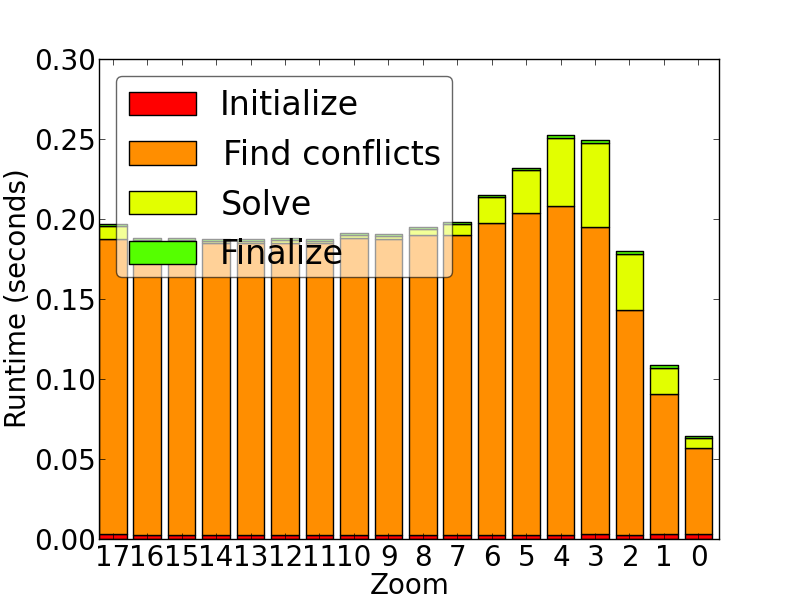
\includegraphics[width=1.0\linewidth]{./figs/prelim_pnt_7k_airports_heuristic_B.png}}
    \centerline{(a) SGA + Proximity}
  \end{minipage} \hfill
  \begin{minipage}{0.329\linewidth}
    \centerline{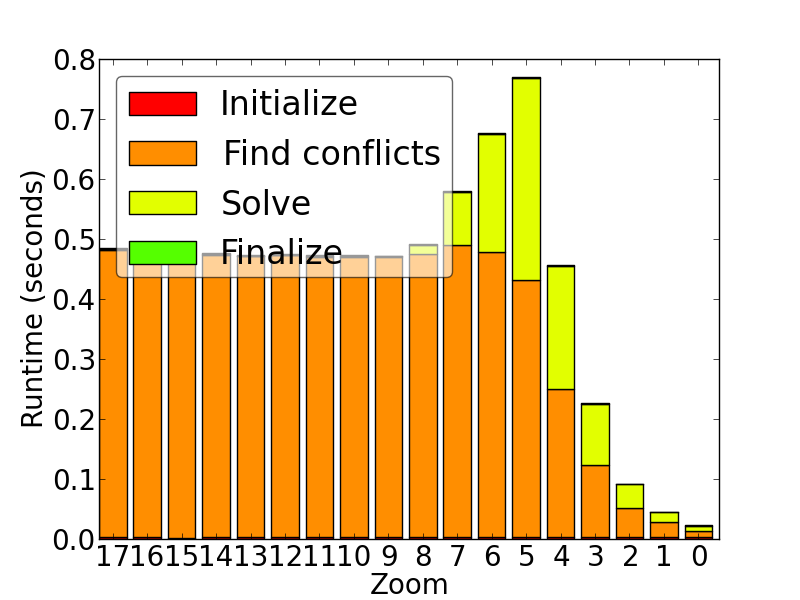
\includegraphics[width=1.0\linewidth]{./figs/prelim_pnt_7k_airports_lp_A.png}}
    \centerline{(b) LPGA + Density}
  \end{minipage} \hfill
  \begin{minipage}{0.329\linewidth}
    \centerline{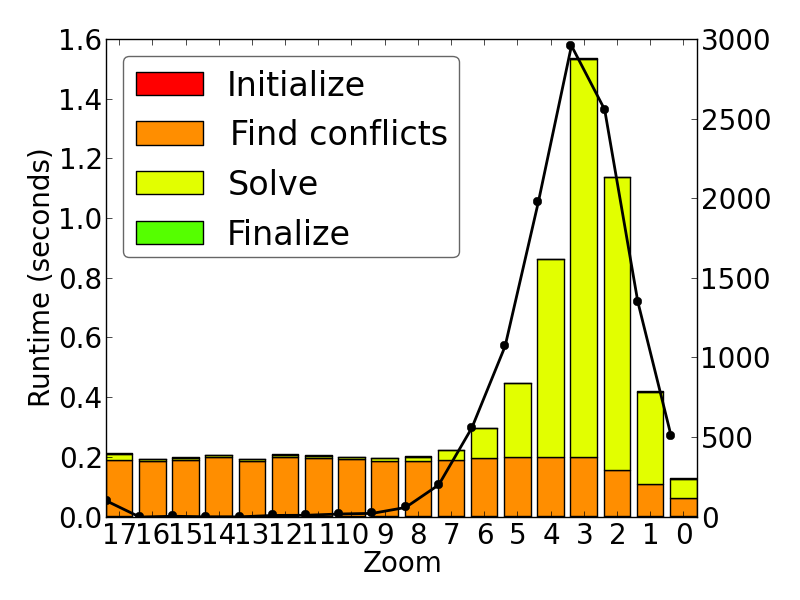
\includegraphics[width=1.0\linewidth]{./figs/prelim_pnt_7k_airports_lp_B.png}}
    \centerline{(c) LPGA + Proximity}
  \end{minipage}
  \vspace{-0ex}
  \caption{Performance breakdown by zoom level, Airport dataset (7K points)} \label{fig:performance:airport}
  \vspace{-2ex}
\end{figure*}

\begin{figure*}[tb]
  \begin{minipage}{0.329\linewidth}
    \centerline{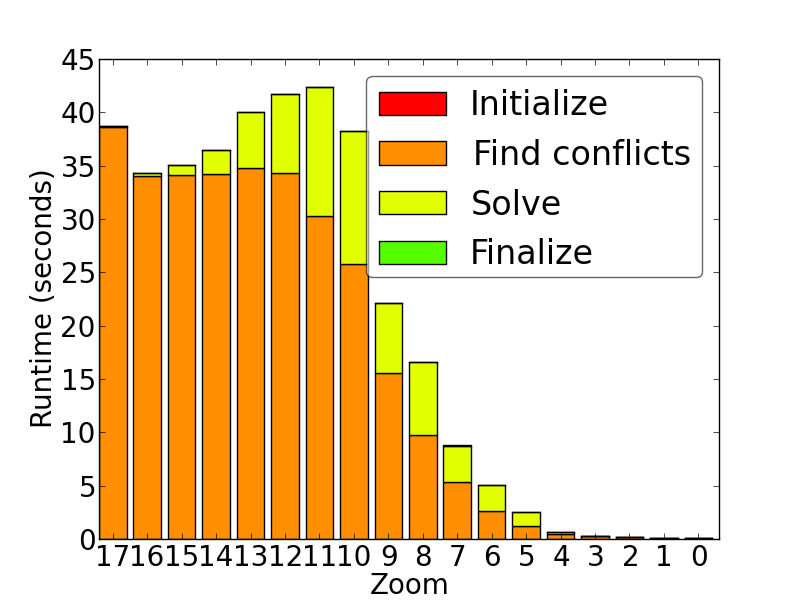
\includegraphics[width=1.0\linewidth]{./figs/prelim_pnt_500k_tourism_heuristic_A.png}}
    \centerline{(a) SGA + Density}
  \end{minipage} \hfill
  \begin{minipage}{0.329\linewidth}
    \centerline{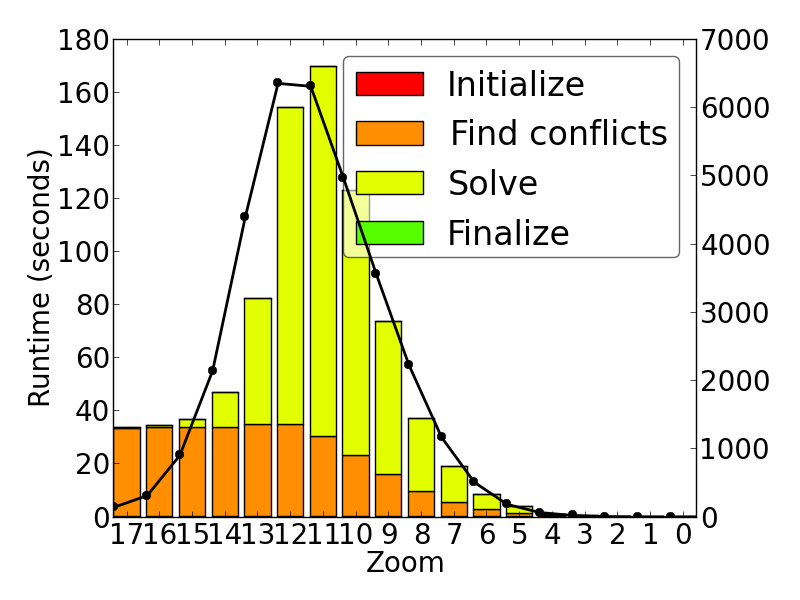
\includegraphics[width=1.0\linewidth]{./figs/prelim_pnt_500k_tourism_lp_A.png}}
    \centerline{(b) LPGA + Density}
  \end{minipage} \hfill
  \begin{minipage}{0.329\linewidth}
    \centerline{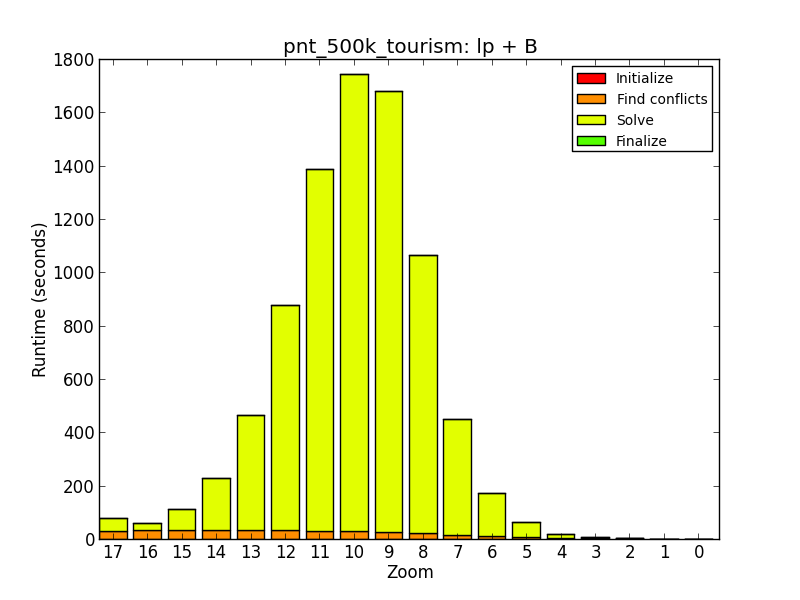
\includegraphics[width=1.0\linewidth]{./figs/prelim_pnt_500k_tourism_lp_B.png}}
    \centerline{(c) LPGA + Proximity}
  \end{minipage}
  \vspace{-0ex}
  \caption{Performance breakdown by zoom level, Tourism dataset (500K points)} \label{fig:performance:tourism}
  \vspace{-2ex}
\end{figure*}

\marcos{We should remove the title from the graph images, and increase the fonts as possible.}

\minisec{Performance and Quality}
 Figure~\ref{fig:performance:airport} shows the performance breakdown per zoom level of executing CVL with the Openflight airports dataset. Note the different y-scales in the graphs. In Parts~(a)-(c), we observe that the time needed to find conflicts is roughly stable until eight zoom levels, then slightly increases, and finally drops sharply for lower zoom levels. The constraints used generate few conflicts at higher zoom levels, given the relatively low density of the airport distribution in space. Nevertheless, even though almost no conflicts are generated, the dataset is still processed, resulting in roughly equal time for finding conflicts and negligible time for solving conflicts per zoom level. 
 
As zoom levels decrease, more conflicts naturally arise, leading initially to increased conflict finding time, as well as conflict solving time. However, as conflicts are solved, records are deleted from the dataset taken as input for the next zoom level. This procedure causes conflict finding time (and eventually total time) to drop significantly for low zoom levels. For SGA under the proximity constraint (Part (a)), total time at zoom level zero is over two times shorter than the initial runtime at zoom level 17; for LPGA under the density constraint (Part (b)), the difference in total time reaches over an order of magnitude.  

Conflict solving time does not increase equally for different solvers. SGA exhibits conflict solving time that is consistently smaller than LPGA. Peak total time for SGA under the proximity constraint (Part (a)) is roughly four times shorter than for LPGA (Part (c)). In addition, LPGA is extremely sensitive to the number of conflicts reported by user-defined constraints. From Parts (b) and (c), we can see that LPGA exhibits peak conflict solving time over three times larger for the proximity constraint than for the density constraint, since the latter generates far fewer conflicts than the former. 

\marcos{Show plot with number of conflicts found per zoom level to support argument above.}

In terms of quality, the difference between SGA and LPGA is not stark. TODO

\marcos{Show quality plots to support arguments above.}

Figure~\ref{fig:performance:tourism} exhibits results with the larger tourism attraction dataset. Since the dataset is denser in space than the airport dataset, conflicts are found and solved at higher zoom levels, resulting in an earlier drop in total time per zoom level. For Parts (a)-(c), total time is uninteresting for zoom levels lower than five. The same cannot be said, however, about peak total time in general, and about conflict solving time in particular.

Parts (a) and (b) compare performance of SGA and LPGA under the density constraint. Even though density generates a smaller number of conflicts than proximity, peak total time for LPGA is still roughly a factor of four larger than for SGA (see zoom level 11). Note that the difference is completely due to the efficiency of the solver, since the time to find conflicts is essentially the same for both methods. Total time for LPGA rises prohibitively when we employ the proximity constraint, reaching a baffling peak of near half an hour at zoom level 10 (Part (c)). While not shown, total times per zoom level for SGA under the proximity constraint are roughly comparable to the times reported in Part (a) for the density constraint using this dataset. SGA's peak total time is slightly above 40 seconds, roughly a factor of 40 smaller than LPGA's.         

While SGA performs significantly better than LPGA, it does not do so at the cost of quality. As discussed in Section~\ref{sec:algorithms:sga}, SGA is optimal for the density constraint, since conflict sets are disjoint. For the proximity constraint, TODO

\marcos{Add quality argument above for SGA vs. LPGA for proximity constraint when we get the numbers.}


\minisec{Scalability}
\marcos{Show scalability plots and discuss main effects; probably they will mostly confirm the effects observed above.}


\subsection{Complex Shape Data}
\label{sec:exp:complex:shapes}

\minisec{Performance and Quality}
\marcos{Show performance and quality plots for linestrings and polygons.}

\minisec{Scalability}
\marcos{Show scalability plot for polygons.}

\subsection{Large-Scale Test}
\label{sec:exp:large}

\marcos{Show resuls with the large-scale dataset with 30M points.}

